\chapter{GAN Vizualizátor}
\label{gan}

Priradenie farby ku skladbe nie je dostačujúce.
Preto sme vytvorili model, ktorý generuje obrázky.
Na vyriešenie tohto problému sme zvolili generatívnu konkurenčnú sieť, spomínanú v predošlých kapitolách.
Ďalej v tejto kapitole opíšeme konkrétny návrh a implementáciu vizualizátora.

\section{Návrh}
Ako sme opísali v kapitole dva, generatívna konkurenčná neurónová sieť je tvorená dvoma sieťami.
V našom návrhu budú generátor tak ako aj diskriminátor tvoriť dopredné neurónové siete.
Generátor na vstupe potrebuje náhodné dáta, šum, z ktorých bude generovať nové obrázky.
Tento šum je v našom prípade vektor náhodných čísel z rozsahu -1 až 1.
Celkový počet rozmerov vektora je závislý od počtu vstupných kanálov.
Prvotný návrh generátora je tvorený dvoma vrstvami.
Prvá vrstva ma 128 neurónov, pričom každý neurón má 100 vstupných kanálov.
Výstupy neurónov druhej vrstvy tvoria celkový výstup siete.
Ich počet je závislý od požadovanej veľkosti generovaných obrázkov.
Nakoľko chceme generovať obrázky veľkosti 64x64, počet neurónov druhej vrstvy je 4096, pričom každý má 128 vstupných kanálov.

Diskriminátor je klasifikátor tvorený tak isto dvomi vrstvami.
Prvá, vstupná vrstva je tvorená 128 neurónmi.
Nakoľko na vstupe je obrázok, u ktorého sa posudzuje reálnosť, počet vstupných kanálov je pre 64x64 obrázok 4096.
Druhá a zároveň výstupná vrstva je tvorená len jedným neurónom s počtom vstupných kanálov totožným s počtom neurónov predošlej vrstvy.
Výstupom tejto vrstvy bude hodnota v intervale 0 až 1, ktorá predstavuje pravdepodobnosť či ide o skutočné dáta.

Trénovanie tohto modelu je náročné nakoľko diskriminačná sieť sa snaží maximalizovať výstupnú pravdepodobnosť, na druhej strane generátor sa túto hodnotu snaží minimalizovať.
Matematicky by sa tento problém dal vyjadriť ako \[\min_{G}\max_{D}V(D,G)\]
\[V(D,G)=E_{x\sim p_{data}(x)}[logD(x)] + E_{z\sim p_{z}(z)}[log(1 - D(G(z)))]\]
, kde prvý člen funkcie je entropia, že dáta zo skutočnej distribúcie prejdú diskriminátorom.
Diskriminátor sa snaží túto hodnotu maximalizovať na 1.
Druhý člen je entropia, že náhodný vstup vojde do generátora, ktorý vygeneruje vstup do diskriminátora.
Generátor sa snaží minimalizovať výstup.

Našťastie objavitelia GAN sietí popisujú vo svojej práci algoritmus na trénovanie tohto modelu \cite{GAN}.
Trénovanie prebieha v troch krokoch:
\begin{enumerate}
	\item Trénovanie diskriminátora na reálnych dátach v niekoľkých epochách.
	\item Vygenerovanie nových dát a prechod diskriminátorom.
	\item Trénovanie generátora za pomoci výstupu z minulého kroku.
\end{enumerate}
Celý tento proces môže prebiehať vo viacerých cykloch.
V pôvodnom algoritme je pre učenie diskriminačnej siete využitý algoritmus gradient ascend.
Chyba pre túto sieť je definovaná ako
\[\frac{1}{m}\sum_{i=1}^{m} [logD(x^{(i)}) + log(1 - D(G(z^{(i)})))]\]
, kde \(m\) je počet vstupných dát alebo inak povedané veľkosť dávky.
Pre generátor, s využitím algoritmu gradient descend, definujeme chybu ako
\[\frac{1}{m}\sum_{i=1}^{m} log(1 - D(G(z^{(i)})))\]

\section{Implementácia}
V prvom rade je nevyhnutné upraviť vstupné dáta.
Pre stručnosť opíšeme úpravu len obrázkov ručne kreslených skíc z nášho datasetu.
Pre detailné obrázky je potrebná podobná úprava len s malými zmenami.
Obrázky na disku sú uložené vo formáte png s hĺbkou 4.
Aj keď sú uložené vo formáte RGB, obsahujú len čiernobiely obraz.
Pozadie týchto obrázkov je nastavené na priehľadné a majú veľkosť 320x320.
Pre našu sieť sú tieto obrázky príliš veľké a majú zlú farebnú hĺbku.
Proces úpravy preto rieši tieto nedostatky.
\begin{minted}{python}
img = Image.open(image_name)
white_back = Image.new('RGB', img.size, (255,255,255))
white_back.paste(img, mask = img.split()[3])

gray = white_back.convert('1')
small = gray.resize((HEIGHT, WIDTH))
arr = np.array(small)
flat_arr = arr.ravel()
return (1*flat_arr)
\end{minted}
Táto funkcia nazačiatku vytvorí nové biele pozadie a spojí ho s existujúcim obrázkom.
Následne je tento obrázok konvertovaný na dvojrozmerné pole jednotiek a núl signalizujúcich biele a čierne pixle.
Ostáva už len zmeniť jeho veľkosť a upraviť dvojrozmerné pole na jednorozmerné.

Obrázky sú po úprave pripravené na vstup do siete nadefinovanej v predchádzajúcej podkapitole.
Podľa návrhu sme naimplementovali model generátora aj diskriminátora v pythone za použitia modulov tensorflow a numpy.
V sieti generátora sme pre prvú vrstvu zvolili aktivačnú funkciu relu, nakoľko ide o odporúčanie viacerých výskumníkov.
Aktivačnú funkciu pre výstupnú vrstvu tvorí sigmoid funkcia, ktorá nadobúda hodnoty medzi 0 a 1.
Diskriminátor je až na zmenu v počte neurónov implementovaný rovnako.

Výpočet chyby sme boli nútený trošku pozmeniť, nakoľko tensorflow nepozná algoritmus gradient ascend.

\begin{minted}{python}
D_loss = -tf.reduce_mean(tf.log(D_real) + tf.log(1. - D_fake))
G_loss = -tf.reduce_mean(tf.log(D_fake))

D_solver = tf.train.AdamOptimizer().minimize(D_loss, var_list=theta_D)
G_solver = tf.train.AdamOptimizer().minimize(G_loss, var_list=theta_G)
\end{minted}

D\_loss v uvedenom kóde predstavuje chybu diskriminátora, z uvedeného dôvodu je zmenená na zápornú a namiesto maximalizovania používame optimalizátor na minimalizáciu.
Takisto chyba generátora nie je totožná s pôvodným vzorcom.
Odôvodnenie je, že v tomto tvare algoritmus dosahuje lepšie výsledky.


\section{Podmienená generatívna sieť}
Zatiaľ náš model dokáže generovať obrázky z náhodnej distribúcie.
Zadaním tejto práce je ale generovať obrázky za pomoci hudby.
Generatívnu konkurenčnú sieť, ktorú sme vytvorili zmeníme na podmienenú GAN alebo CGAN (ang. conditional generative adversarial network).
CGAN na rozdiel od GAN na vstupe do generatívnej aj diskriminatívnej siete potrebuje aj nový štítok (ang. label), ktorý nesie nejakú informáciu pre požadovaný výstup.
Naše siete sa zmenia z \(G(z)\) a \(D(X)\) na \(G(z,y)\) a \(D(X,y)\).

Z matematického pohľadu \(G(z,y)\) modeluje distribúciu našich dát pri zadaní \(z\) a \(y\).
To znamená, že vzorec na generovanie dát je 
\[X\sim G(X|z,y)\]
Podobne pre diskriminátor, ktorý sa snaží nájsť pravdepodobnosť reálnosti pre \(X\) a \(X_{G}\), výsledky dostávame ako
\[d\sim D(d|X,y)\]
Čiže funkcia pre požadovaný výsledok nášho modelu so započítaním nových skutočností je
\[\min_{G}\max_{D}V(D,G)=E_{x\sim p_{data}(x)}[logD(x,y)] + E_{z\sim p_{z}(z)}[log(1 - D(G(z,y),y))]\]
V našom prípade tvoria vektor \(y\), z danej rovnice, naše hudobné dáta.
Vstup hudobnej informácie do neurónovej siete sme opísali v kapitole päť.

\section{Zmena parametrov}
Pravdepodobnosť, že náš navrhnutý model dokáže generovať obrázky v požadovanej kvalite je veľmi malá.
Úprava všetkých parametrov siete, ako sú počet neurónov vo vrstvách, rýchlosť učenia alebo typ optimalizátora sa nedá automatizovať. 
\begin{figure}[!ht] 
	\centering 
	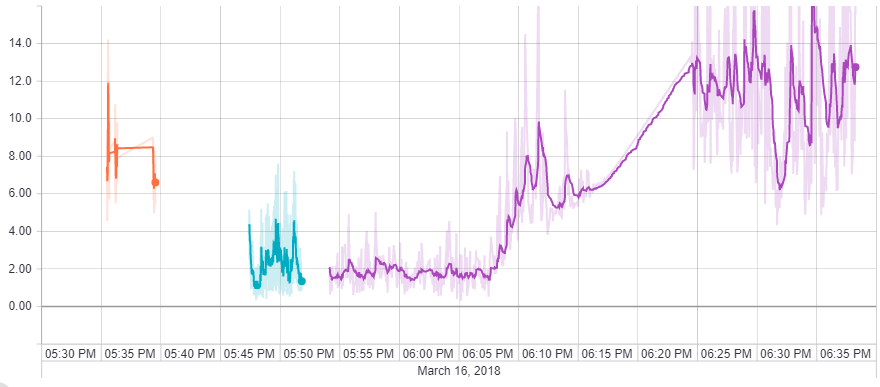
\includegraphics[width=.8\textwidth]{figures/g_loss_1} 
	\caption{Chyba generátora pri trénovaní neoptimalizovanej siete.} 
	\label{g_loss_1}
\end{figure}

Bez optimalizovania boli výsledky nášho modelu hudobného vizualizátora, tak ako sme predpokladali, nedostačujúce.
Na obrázku \ref{g_loss_1} sú zaznamenané tri trénovania, v rôznych časoch a trvaniach, na skicách z nášho datasetu.
Je vidno že strata generátora po prvých dvoch trénovaniach klesla, no potom sa klesanie zastavilo dokonca trénovanie úplne zlyhalo a chyba začala rapídne divergovať.
Náraz chyby spôsobil zmenu váh siete na neprípustné hodnoty, čo pri ďalšej epoche trénovania viedlo k nekonečným alebo neznámim hodnotám chýb obydvoch sietí.
Tieto hodnoty tensorflow nedokáže spracovať a program trénovania spadol.
Z toho dôvodu všetky naše ďalšie kroky smerovali k stablizácií trénovania.

V prvom rade sme normalizovali vstupné dáta.
Jednou časťou normalizácie je zmenšenie každej vzorky  o priemernú hodnotu vypočítanú zo vzoriek danej vlastnosti.
Druhou časťou je min-max normalizácia, pri ktorej každú vlastnosť danej vzorky upravíme na hodnotu z intervalu \(<-0,5; 0,5>\).
Trénovanie týchto dát bolo možné udržať dlhšie ale problém nebol úplne eliminovaný.

S predpokladom, že problém tkvie v typológií siete, sme zmenili počet vrstiev.
Nový generátor mal vstupnú vrstvu so 128 neurónmi, dve skryté vrstvy so 128 a 512 neurónmi a výstupnú vrstvu.
Na výstupe sa aktivovala sigmoind funkcia všade inde relu.
Diskriminátor ostal nezmenený, nakoľko sme predpokladali, že lepší generátor bude mať výhodu nad diskriminátorom, čo by viedlo k poklesu chyby.
Táto zmena nepriniesla žiaden pozitívny výsledok.
Je známim faktom, že aktivačná funkcia leaky relu má lepšie výsledky ako relu.
Implementovali sme túto funkciu a využili v generátore.

\begin{minted}{python}
def lrelu(x, alpha):
    return tf.nn.relu(x) - alpha * tf.nn.relu(-x)
\end{minted}

Nevedli sme si poradiť s výpadkami programu, tak sme pristúpili k riadenému trénovaniu sietí.
Snahou bolo zabrániť chybe generátor presiahnúť vysokú hodnotu.
Z toho dôvodu sme dovolili trénovať diskriminátor len v prípade, že chyba generátora je menšia ako 4.
Daná úprava dovoľovala generátoru dobehnúť diskriminátor a program už nespadol.
Výsledky trénovania však neboli pozitívne.

Keď už sme mohli trénovať aj v dlhších časových úsekoch, začali sme viac experimentovať s parametrami siete.
Zväčšili sme diskriminátor, zmenili aktivačné funkcie či upravili mieru trénovania v algoritme gradient descent.
Nič z toho neprinieslo požadovaný úspech.

Pri hľadaní riešenia na otázku stabilizovania GAN siete, sme narazili na iný prístup k výpočte chyby.
Nový výpočet spočíval vo výpočte tzv. wasserstein distance.
Upravili sme diskriminátor aby na výstupe nebola aktivačná funkcia.
Zmenili sme výpočty chýb na:

\begin{minted}{python}
D_loss = tf.reduce_mean(D_real) - tf.reduce_mean(D_fake)
G_loss = -tf.reduce_mean(D_fake)
\end{minted}

Použili sme menšiu mieru trénovania a nechali trénovať diskriminátor viac.
\begin{minted}{python}
for _ in range(5):
	D_summary, _, D_loss_curr, _ = sess.run(
		[D_merge, D_solver, D_loss, clip_D], 
		feed_dict={X: X_mb, Z: sample_Z(mb_size, z_dim), y:y_mb}
	)

G_summary, _, G_loss_curr = sess.run(
	[G_merge, G_solver, G_loss], 
	feed_dict={Z: sample_Z(mb_size, z_dim), y:y_mb}
)
\end{minted}

Táto zmena stabilizovala trénovanie.
Program nespadol a nebolo nutné zasahovať manuálne do algoritmu.
Pre porovanie sme vyskúšali dva optimalizátory, konkrétne AdamOptimizer a RMSPropOptimizer.

\begin{figure}[!ht] 
	\centering 
	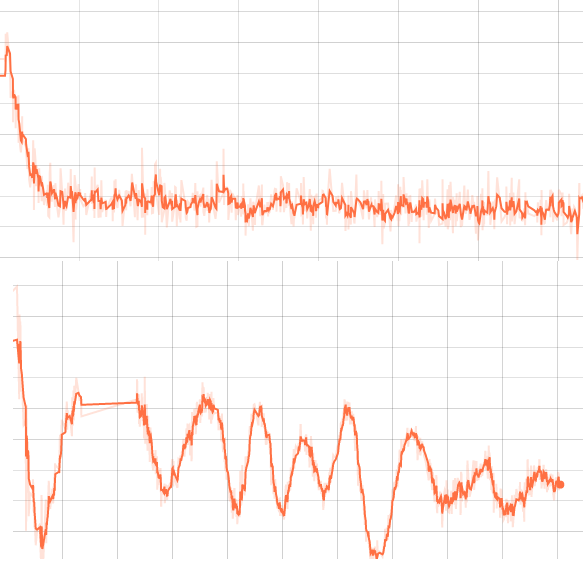
\includegraphics[width=.4\textwidth]{figures/adam_vs_rms} 
	\caption{Chyba diskriminátora pri využití RMSPropOptimizer (hore) a AdamOptimizer (dole).}
	\label{a_vs_r}
\end{figure}

Chyba diskriminátora konvergovala rýchlejšie ako je vidieť na obrázku \ref{a_vs_r}, tak sme sa rozhodli využívať pri ďalšom trénovaní už len tento optimalizátor.
Opäť sme vyskúšali niekoľko typov siete.
Najlepšie výsledky sme dosiahli pri Generátore, ktorý využíval Leaky ReLu aktivačné funkcie na skrytých vrstvách a Sigmoid funkciu na výstupe.
Diskriminátor v tomto modely mal presne opačnú topológiu v porovnaní s generátorom a ako ativačné funkcie využíval ReLu.
Táto GAN sieť dokázala generovať obrázky podobné nášmu datasetu, pri zadaní piesne z datasetu.
Ak však na vstupe bola skladba, ktorú sieť pri trénovaní nemala, výstup bol bez kontextu.

Tento problém sme sa snažili vyriešiť využitím iného datasetu, ktorý obsahoval menšie množstvo akustických vlastností pri jednotlivých vzorkách.
Ani po veľmi dlhom trénovaní výsledky neboli pre nás dostatočné.
Posledným krokom, ktorým sme sa snažili vylepšiť výsledok, bolo zakomponovanie konvolučných vrstiev do siete.
Vytvorli sme generátor, ktorý pozostával z dvoch konvolučných vrstiev.
Výsledky toho modelu naznačovali, že pre generovanie správnych obrázkov potrebujeme viac konvolúcií.
Rozmery takej siete by, ale náš stroj nezniesol a tak sme od tohto riešenia ustúpili.

\section{Zväčšovanie obrázkov}
Hudobný vizualizátor popísaný v tejto kapitole je teoreticky schopný produkovať obrázky ľubovoľnej veľkosti.
Veľkosť ale musí byť zadaná predom, čo nám znemožňuje akúkoľvek neskoršiu manipuláciu s rozmermi bez strát a rozmazania.
Samozrejme rozmery závisia aj od obrázkov v datasete.
Čo sa týka samotného algoritmu, nič nás neobmedzuje vo vytvorení vhodného setu dát a generovania obrázkov vo vysokom rozlíšení.
Prakticky sme ale obmedzený operačnou pamäťou a výpočtovým výkonom.
Z toho dôvodu je možné generovať len malé rozlíšenia.

Pre zväčšovanie obrázkov by sme mohli požiť nejaký algoritmus na zaostrovanie, no tie neprodukujú dostatočne ostré obrazy.
Namiesto toho využijeme Kompozitnú vzory vytvárajúcu sieť (ang. Compositional pattern-producing network).
Využijeme skript vytvorený Liviu Pirvanonm.
Ním navrhnutá sieť sa dokáže naučiť štruktúru jedného obrázka a podľa nej dokáže generovať nové obrázky ľubovoľných rozmerov.
Táto CPPN sieť na vstupe berie súradnice jednotlivých pixlov.
Na výstupe sa snaží určiť správnu farbu pre zadané súradnice.
Celá sieť tak funguje ako funkcia, ktorá aproximuje obrázok.
Keďže vykresľuje po jednotlivých pixloch, tak veľkosť vykreslených obrázkov môže byť ľubovoľná a je obmedzená len operačnou pamäťou.
Takto môžeme naše výstupy z CGAN vizualizátora o veľkosti 64x64 prekonvertovať aj na rozlíšenia 4K a viac.
Samozrejme, že táto konverzia nie je dokonalá a stojí relatívne veľa času kvôli nutnosti trénovania siete pre každý obrázok zvlášť.
Nové obrázky sú síce rozmazané ale majú o niečo lepšiu kvalitu ako, keby boli zväčšené klasickým spôsobom.

\begin{figure}[!ht] 
	\centering 
	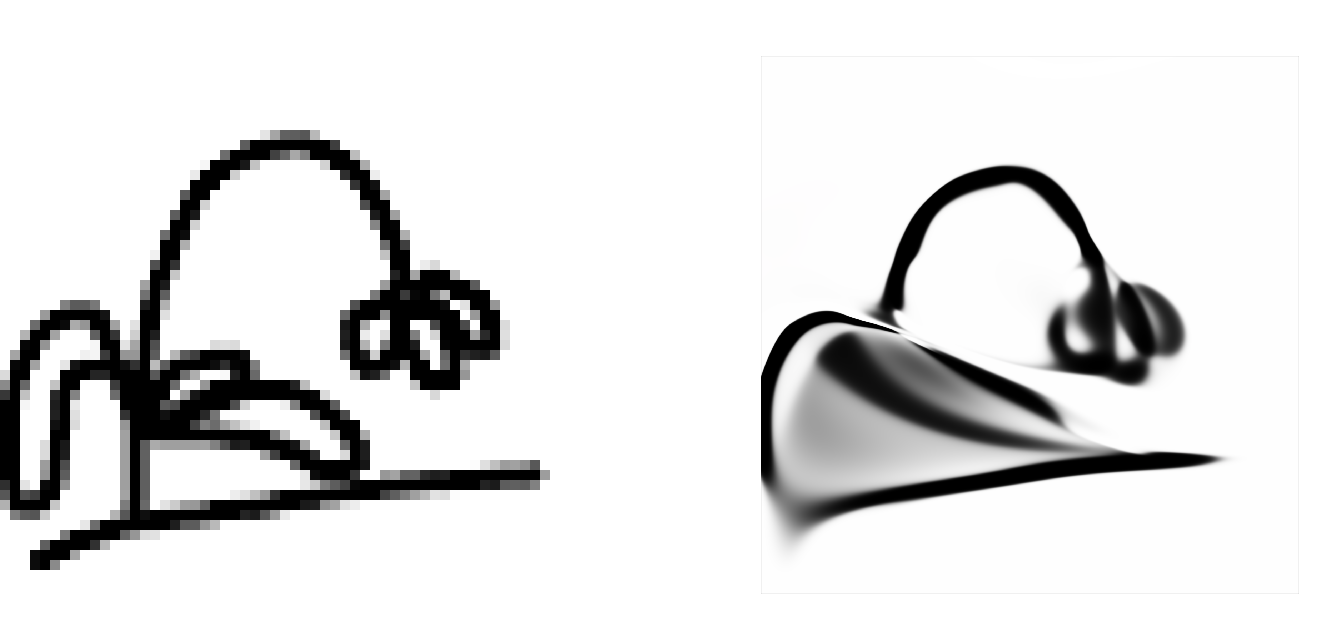
\includegraphics[width=.8\textwidth]{figures/cppn} 
	\caption{Zväčšenie obrázku z datasetu využitím CPPN siete.}
	\label{cppn}
\end{figure}

Funkčnosť tejto neurónovej siete sme overili na jednom obrázku z nášho datasetu.
Výsledok je možné vidieť na obrázku \ref{cppn}.
Vľavo sa nachádza pôvodný obrázok vo veľkosti 64x64 zväčšený klasickým spôsobom na veľkosť 640x640.
Vpravo je vygenerovaný obrázok pomocou CPPN siete vo veľkosti 2048x2048.
